\documentclass[11pt,a4paper]{article}

\usepackage[utf8]{inputenc}
\usepackage[T1]{fontenc}
\usepackage[english]{babel}
\usepackage[margin=2.5cm]{geometry}
\usepackage{amsmath,amssymb}
\usepackage{graphicx}
\graphicspath{{figures/}{../figures/}}
\usepackage{booktabs}
\usepackage{forest}
\usepackage[hidelinks]{hyperref}

\title{Quantitative Information Flow in Subliminal Learning}
\author{Author 1 \and Author 2 \and Author 3}
\date{\today}

\begin{document}
\maketitle

\section{Introduction}
Subliminal learning occurs when a language model (the \emph{student}) is
fine-tuned on data generated by another language model (the \emph{teacher})
and acquires a behavioral trait of the teacher, even though the data have
no apparent semantic connection to that trait. For example, a teacher
with an induced animal preference can transmit it to a student through
numerical sequences containing no explicit mention of the
animal~\cite{cloud2025}. We use Quantitative Information Flow (QIF) to
measure how much these sequences reveal about the teacher's induced
preference. We compare exact channel computation with Monte Carlo
estimation and investigate how leakage and computational cost vary with
the observations available to an adversary.

\section{Channel Model}
The secret $X$ describes the teacher's preference condition, the observation
$Y$ is its generated numerical continuation, and $p$ is a fixed public prompt:
\[
  C_{x,y}=P(Y=y\mid X=x,p).
\]
Two possible secret spaces are multiple induced preferences, such as
$\mathcal X=\{\text{owl},\text{cat},\text{dog}\}$, or a binary comparison,
$\mathcal X=\{\text{no induced preference},\text{dog preference}\}$.
Preferences can be induced through prompting or fine-tuning, with the
unmodified model serving as the control in the binary setting. In either
case, we assign a uniform prior $\pi_x=1/|\mathcal X|$ over the secrets.

\section{Leakage Measurement}
The prior and posterior Bayes vulnerabilities are
\[
  V_1(\pi)=\max_x\pi_x,
  \qquad
  V_1(\pi,C)=\sum_y\max_x\pi_x C_{x,y}.
\]
They represent the optimal probability of guessing the secret before
and after observing the channel output, respectively.

\section{Methods}
\subsection{Exact Channel with Restricted Outputs}
We computed the restricted channel for continuations of the fixed prefix
``182, 818, 725'', consisting of two integers from $100$ to $999$ separated
by a comma and a space. Excluding leading zeros gives
\[
    |\mathcal Y|=(9\cdot10\cdot10)^2=810{,}000.
\]
At each digit position, we normalize the logits over the allowed digits;
separators are forced. The implementation checks that each digit is a
single token. The resulting probabilities are exact for this masked
procedure, rather than for unrestricted generation.

\paragraph{Computing the channel efficiently.}
For the six generated digits $y=(y_1,\ldots,y_6)$, the channel probability is
\[
    C_{x,y}=\prod_{t=1}^{6}P(y_t\mid y_{<t},x,p),
\]
where the context includes the forced separator when applicable.
We enumerate distinct digit prefixes by depth and propagate their
probabilities, sharing each next-digit distribution across all its
continuations. The following binary example illustrates this prefix tree:

\begin{center}
\begin{forest}
for tree={
    draw,
    rounded corners,
    inner sep=3pt,
    l sep=10pt,
    s sep=6pt
}
[$\varepsilon$
    [$0$
        [$00$
            [$000$]
            [$001$]
        ]
        [$01$
            [$010$]
            [$011$]
        ]
    ]
    [$1$
        [$10$
            [$100$]
            [$101$]
        ]
        [$11$
            [$110$]
            [$111$]
        ]
    ]
]
\end{forest}
\end{center}

Here, $\varepsilon$ is the empty prefix: both $000$ and $001$ use the
same next-digit distribution after $00$. In our restricted channel,
the branching factors are $(9,10,10,9,10,10)$, requiring
\[
    N_{\text{prefixes}}
    =1+9+90+900+8{,}100+81{,}000=90{,}100
\]
next-digit distributions per teacher. Prefixes are processed in batches.
The implementation reuses the prompt's \textit{KV cache}, but reprocesses
the numerical prefix at each depth rather than retaining an incremental
cache for every branch.

\subsection{Monte Carlo Estimation Using Logits}
For free-form generation the output space cannot be enumerated, but the
posterior Bayes vulnerability is an expectation over the marginal
$P(y)=\sum_x\pi_xC_{x,y}$:
\begin{equation}\label{eq:expectation}
  V_1(\pi,C)=\sum_y P(y)\max_x P(x\mid y)
  =\mathbb E_{y\sim P(y)}\Big[\max_x P(x\mid y)\Big],
  \qquad
  P(x\mid y)=\frac{\pi_xC_{x,y}}{\sum_{x'}\pi_{x'}C_{x',y}}.
\end{equation}
It is therefore estimated without bias by the sample mean
\[
  \hat V_1=\frac1N\sum_{j=1}^{N}\max_x P\big(x\mid y^{(j)}\big),
  \qquad y^{(j)}\sim P(y).
\]
To sample from $P(y)$, each round first draws a teacher from the prior and then
lets it generate a sequence; generating every sequence from the same teacher
would estimate a different quantity. The posterior requires $C_{x,y}$ under
\emph{every} teacher. For a language model this is the product of next-token
probabilities, which teacher forcing computes exactly from the logits:
\[
  C_{x,y}=\prod_{t=1}^{L}P_{\theta_x}\!\left(y_t\mid p,\,y_{<t}\right).
\]
If the adversary observes $k$ sequences from the same teacher (the parallel
composition $C^{(k)}$), their likelihoods multiply. We report a normal 95\%
interval, which covers Monte Carlo variability only. The estimate is valid
only if sequences are generated from the same distribution that is used to score
them. The synthetic and Qwen free-generation experiments use temperature
$1$ without top-$k$, top-$p$ or repetition penalty and no filtering.
For Gemma, we also estimate the channel conditioned on acceptance by the
numerical parser, accounting for teacher-dependent acceptance probabilities.

\section{Experiments and Results}
We evaluate estimation accuracy, computational cost and the relationship
between leakage and behavioral transfer.

\paragraph{Scaling exact-channel computation.}
We measured exact-channel enumeration time as the number of observed digits
increased, using Qwen2.5-7B-Instruct on one L40S.
Figure~\ref{fig:exact-timing} shows the measurements and projections for
longer outputs: despite prefix reuse, exponential growth quickly makes
enumeration impractical.

\begin{figure}[htbp]
\centering
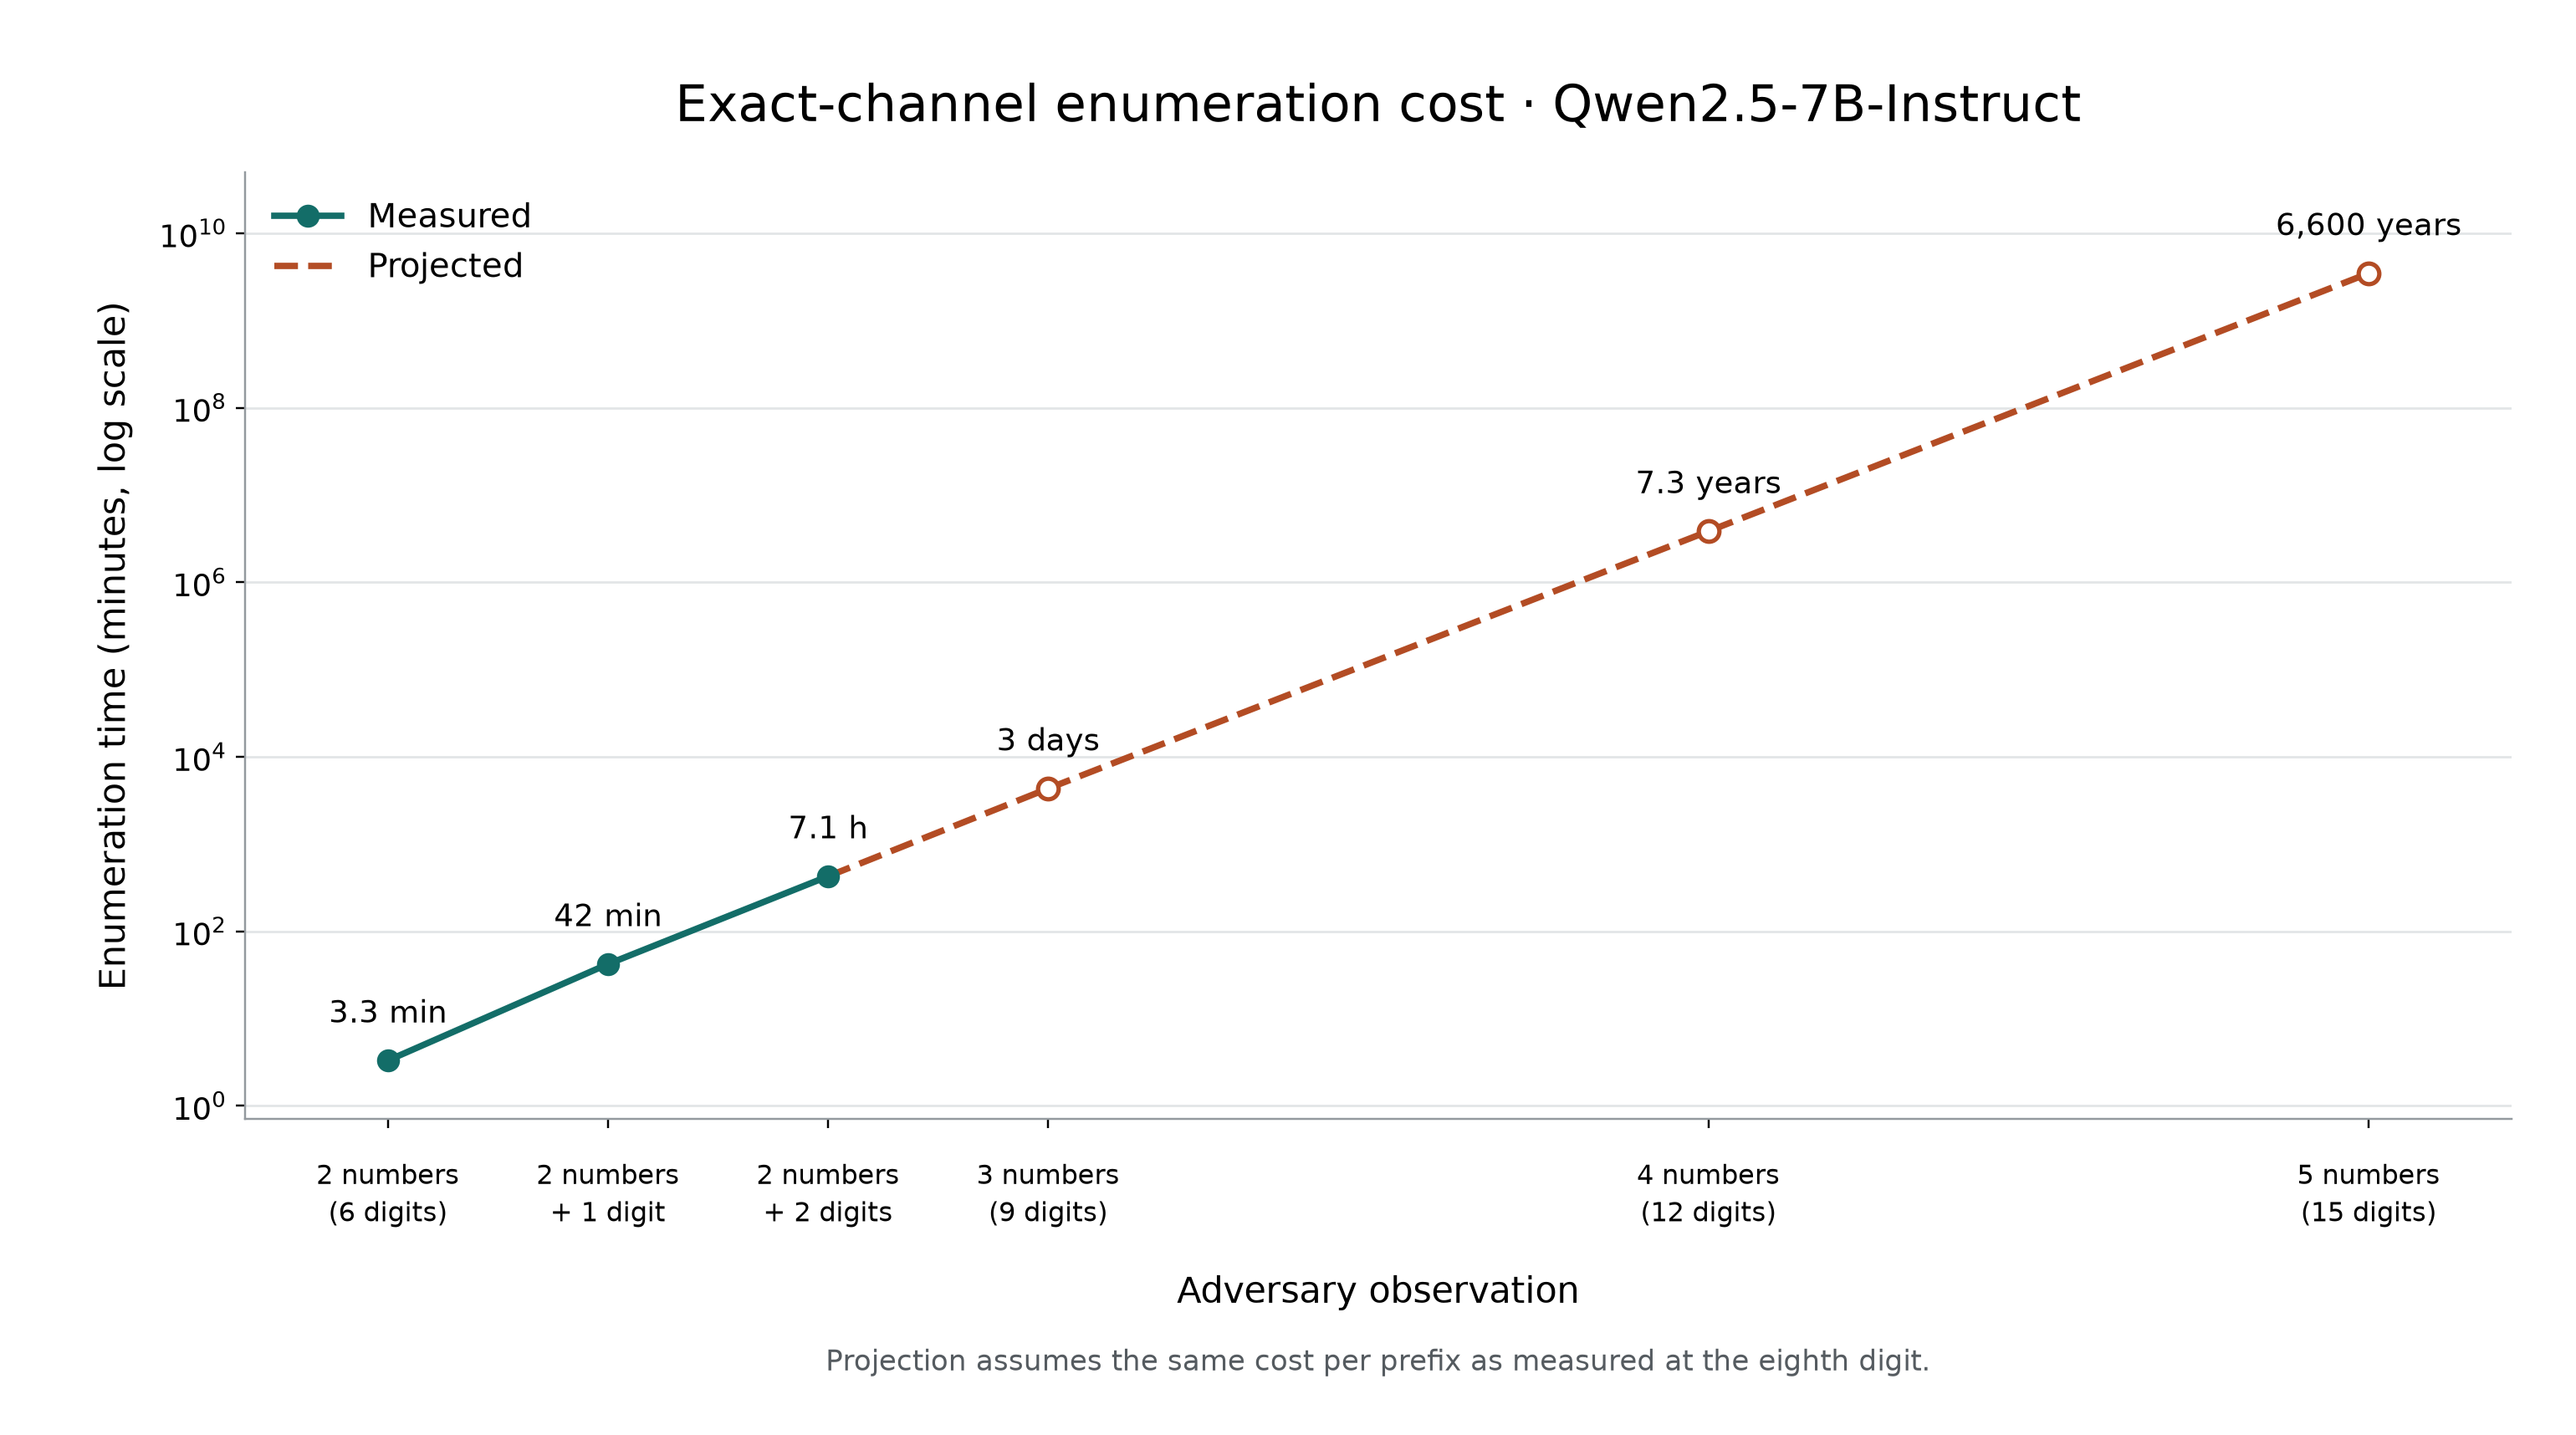
\includegraphics[width=0.9\linewidth]{exact_channel_timing_en.png}
\caption{Exact-channel enumeration time on one L40S, excluding model loading.
Solid points are measured; hollow points extrapolate a constant marginal
cost per prefix from the eighth digit.}
\label{fig:exact-timing}
\end{figure}

\paragraph{Synthetic teachers.}
To compare Monte Carlo with an exact value, we use three teachers whose tokens
are i.i.d.\ over $\{0,1,2,3\}$; each gives probability $0.55$ to its own digit
and $0.15$ to the others. With a fixed length $L$ there are $4^L$ sequences, so
$V_1$ can be enumerated. We use $L\in\{1,2,4\}$, $k\in\{1,2,4,8\}$ lists with
$L=2$, a uniform prior and $N=20{,}000$ rounds.

\paragraph{Validation.}
On the synthetic teachers the exact value lies inside the Monte Carlo interval
for every length (Table~\ref{tab:validation}). On Qwen2.5-0.5B, the
log-probabilities computed by teacher forcing match those reported during
generation to within $5\times10^{-5}$, so generation and scoring use the same
distribution.

\begin{table}[h]
\centering
\small
\begin{tabular}{@{}rrrcc@{}}
\toprule
Length $L$ & $|\mathcal Y|$ & Exact $V_1(\pi,C)$ & Monte Carlo $\hat V_1$ & 95\% interval \\
\midrule
1 & 4   & 0.6000 & 0.5987 & [0.5972, 0.6003] \\
2 & 16  & 0.6400 & 0.6412 & [0.6386, 0.6439] \\
4 & 256 & 0.7624 & 0.7638 & [0.7612, 0.7664] \\
\bottomrule
\end{tabular}
\caption{Exact and Monte Carlo posterior Bayes vulnerability for the synthetic
teachers (prior vulnerability $1/3$).}
\label{tab:validation}
\end{table}

\paragraph{Qwen2.5-0.5B teachers.}
The teachers are Qwen2.5-0.5B-Instruct with the system prompt ``You love
owls.\ You think about owls all the time.'' and its cat and dog versions. The
public prompt asks for ten three-digit numbers after ``182, 818, 725,'', and
generation stops at the end-of-sequence token or after $40$ tokens. We run
$120$ rounds with one list and $120$ with three lists. As a control, three
identical teachers (``You love animals.'') must give exactly the prior, $1/3$.

\paragraph{Leakage of Qwen2.5-0.5B teachers.}
The identical-teacher control gives exactly the prior, so the estimator does not
create leakage by itself. For the animal teachers, one list raises the optimal
probability of guessing the preference from $0.333$ to $0.391$, and three lists
to $0.436$ (Table~\ref{tab:qwen}). The preference leaks, but little: the
posterior stays close to uniform for any single list.

\begin{table}[h]
\centering
\small
\begin{tabular}{@{}lrrcrr@{}}
\toprule
Condition & Rounds & $\hat V_1(\pi,C)$ & 95\% interval & $\mathcal L^{\times}_1$ & $\mathcal L^{+}_1$ \\
\midrule
prior (no observation)       & --- & 0.333 & ---            & 1.000 & 0.000 \\
identical teachers (control) &  20 & 0.333 & [0.333, 0.333] & 1.000 & 0.000 \\
one list                     & 120 & 0.391 & [0.384, 0.398] & 1.172 & 0.057 \\
three lists                  & 120 & 0.436 & [0.423, 0.448] & 1.307 & 0.102 \\
\bottomrule
\end{tabular}
\caption{Posterior Bayes vulnerability of the owl, cat and dog teachers
(Qwen2.5-0.5B), with multiplicative and additive leakage.}
\label{tab:qwen}
\end{table}

\paragraph{Sequence length and several lists.}
Leakage grows with the observed data. On the synthetic teachers it grows with
the sequence length (Table~\ref{tab:validation}) and with the number of lists:
$\hat V_1=0.640$, $0.764$, $0.880$ and $0.965$ for $k=1,2,4,8$. On Qwen the
increase from one to three lists is much smaller ($0.391\to0.436$), consistent
with teachers that differ only by a system prompt.

\paragraph{Computational cost.}
The cost grows linearly with the number of rounds, lists and teachers, and does
not depend on the size of the output space. On a laptop, excluding model
loading, the Qwen2.5-0.5B runs took $83$~s for $120$ rounds with one list and
$242$~s with three lists.

\paragraph{Gemma: prompting versus fine-tuning.}
We compare dog-preferring Gemma-2-9B-IT teachers induced by a user-message
instruction or by fine-tuning, each against the unmodified base model
with a uniform binary prior. Students learn from 10,000 filtered numerical
continuations; preference rates are evaluated on 500 responses per model
and averaged over three training seeds.

With 1,000 Monte Carlo samples and one observed list, we estimate
vulnerability before and after filtering (Table~\ref{tab:gemma}). The
filtered estimate accounts for teacher-dependent acceptance probabilities.
Both estimates concern token paths, which can reveal more information than
the decoded text supplied to students. Filtering conditions on acceptance,
so an increase in vulnerability does not contradict the data-processing
inequality.

\begin{table}[htbp]
\centering
\small
\begin{tabular}{@{}lrrrrrr@{}}
\toprule
Induction & Raw $\hat V_1$ & Filtered $\hat V_1$ & Teacher & Student & Control & $\Delta$ (pp) \\
\midrule
Prompt      & 0.9284 & 0.9045 & 57.2\%  & 8.47\%  & 5.27\% & +3.20 \\
Fine-tuning & 0.9971 & 0.999998 & 100\% & 16.93\% & 6.67\% & +10.27 \\
\bottomrule
\end{tabular}
\caption{Gemma dog-preference rates and posterior vulnerability (prior $0.5$).
Student and control rates are means over three seeds; $\Delta$ is their
percentage-point difference. Filtered vulnerability refers to accepted token paths.}
\label{tab:gemma}
\end{table}

Fine-tuning yields both higher vulnerability and a larger mean transfer
than prompting. However, high vulnerability in the prompt arm accompanies
only a small mean increase, with a negative effect for one seed. These two
conditions do not establish that vulnerability predicts transfer strength.


\section{Conclusion}

\begin{thebibliography}{1}
\bibitem{cloud2025}
A.~Cloud et al.
\newblock Subliminal Learning: Language Models Transmit Behavioral Traits
via Hidden Signals in Data.
\newblock arXiv:2507.14805, 2025.
\end{thebibliography}

\end{document}
